\documentclass[12pt, oneside, titlepage]{article}   	% use "amsart" instead of "article" for AMSLaTeX format

\usepackage{graphicx}
\graphicspath{ {\string} }
\usepackage{subcaption}

%%%%%%%%%%%%%%%%%%%%%%%%%%%%%%%%%%%%%%%%%%%%%%%%%%%%
% set up packages
%%%%%%%%%%%%%%%%%%%%%%%%%%%%%%%%%%%%%%%%%%%%%%%%%%%%
\usepackage{geometry}                
\usepackage{textcomp}                
\usepackage{amsmath}                
\usepackage{graphicx}                
\usepackage{amssymb}                
\usepackage{fancyhdr}                
\usepackage{subcaption}                
\usepackage{bm}                
\usepackage{lineno}

\usepackage[superscript,noadjust]{cite} % puts dash in citations to abbreviate
\usepackage [autostyle, english = american]{csquotes} % sets US-style quotes

\usepackage{etoolbox} % block quotes

\usepackage{float}
\usepackage{color}

\usepackage{pgf}
\usepackage{tikz}
\usepackage{eqnarray}

\usepackage{listings} % code blocks
\usepackage{setspace}

\usepackage{lscape}

\usepackage{natbib}
\bibliographystyle{abbrvnat}
\setcitestyle{authoryear,open={(},close={)}}

%%%%%%%%%%%%%%%%%%%%%%%%%%%%%%%%%%%%%%%%%%%%%%%%%%%%
% call packages
%%%%%%%%%%%%%%%%%%%%%%%%%%%%%%%%%%%%%%%%%%%%%%%%%%%%	
\geometry{letterpaper, marginparwidth=60pt} % sets up geometry              		
\linenumbers % adds line numbers 
\MakeOuterQuote{"} % sets quote style
\doublespacing % setspace

%%%%%%%%%%%%%%%%%%%%%%%%%%%%%%%%%%%%%%%%%%%%%%%%%%%%
% patches with etoolbox 
%%%%%%%%%%%%%%%%%%%%%%%%%%%%%%%%%%%%%%%%%%%%%%%%%%%%	
% block quotes
\AtBeginEnvironment{quote}{\small}

% linenumbers
\makeatletter
\patchcmd{\@startsection}{\@ifstar}{\nolinenumbers\@ifstar}{}{}
\patchcmd{\@xsect}{\ignorespaces}{\linenumbers\ignorespaces}{}{}
\makeatother

%%%%%%%%%%%%%%%%%%%%%%%%%%%%%%%%%%%%%%%%%%%%%%%%%%%%
% tikzlibrary modifications
%%%%%%%%%%%%%%%%%%%%%%%%%%%%%%%%%%%%%%%%%%%%%%%%%%%%	
\usetikzlibrary{fit}
\usetikzlibrary{positioning}
\usetikzlibrary{arrows}
\usetikzlibrary{automata}

%%%%%%%%%%%%%%%%%%%%%%%%%%%%%%%%%%%%%%%%%%%%%%%%%%%%
% page formatting; exact 1 in margins
%%%%%%%%%%%%%%%%%%%%%%%%%%%%%%%%%%%%%%%%%%%%%%%%%%%%
\pagestyle{plain}                                                     

\setlength{\textwidth}{6.5in}    
\setlength{\oddsidemargin}{0in}
\setlength{\evensidemargin}{0in}
\setlength{\textheight}{8.5in}
\setlength{\topmargin}{0in}
\setlength{\headheight}{0in}
\setlength{\headsep}{0in}
\setlength{\footskip}{.5in}

%%%%%%%%%%%%%%%%%%%%%%%%%%%%%%%%%%%%%%%%%%%%%%%%%%%%
% defining code blocks using listings package
%%%%%%%%%%%%%%%%%%%%%%%%%%%%%%%%%%%%%%%%%%%%%%%%%%%%

\definecolor{dkgreen}{rgb}{0,0.6,0}
\definecolor{gray}{rgb}{0.5,0.5,0.5}
\definecolor{mauve}{rgb}{0.58,0,0.82}

\lstset{frame=tb,
  language=R,
  aboveskip=3mm,
  belowskip=3mm,
  showstringspaces=false,
  columns=flexible,
  basicstyle={\small\ttfamily},
  numbers=none,
  numberstyle=\tiny\color{gray},
 % keywordstyle=\color{blue},
  commentstyle=\color{dkgreen},
  stringstyle=\color{mauve},
  breaklines=true,
  breakatwhitespace=true,
  tabsize=3,
  otherkeywords={0,1,2,3,4,5,6,7,8,9},
  deletekeywords={data,frame,length,as,character,dunif,ps},
}

%%%%%%%%%%%%%%%%%%%%%%%%%%%%%%%%%%%%%%%%%%%%%%%%%%%%
%%%%%%%%%%%%%%%%%%%%%%%%%%%%%%%%%%%%%%%%%%%%%%%%%%%%
% begin document
%%%%%%%%%%%%%%%%%%%%%%%%%%%%%%%%%%%%%%%%%%%%%%%%%%%%
%%%%%%%%%%%%%%%%%%%%%%%%%%%%%%%%%%%%%%%%%%%%%%%%%%%%

\begin{document}

% TITLE PAGE
\begin{titlepage}
   \begin{center}
       \vspace*{1cm}
 
       \textbf{Seed banks in \textit{Clarkia xantiana}}
 
       \vspace{1.5cm}
 
       Gregor-Fausto Siegmund and Monica Geber
 
   	Last updated: \today
 
   \end{center}
\end{titlepage}
%


\bibliographystyle{plainnat} 


\section*{Introduction}

Seed banks have important consequences for population persistence by acting as a buffer against environmental change and population stochasticity (\cite{eager2014,paniw2017}), increasing effective population size (\cite{nunney2002,waples2006}), and genetic diversity (\cite{mccue1998b}). The presence of a seed bank can also affect the outcome of evolution (\cite{heinrich2018,ritland1983}). Theory thus suggests that seed banks have ecological and evolutionary consequences (\cite{evans2005}). 

A previous study suggests that the soil seed bank is important for population dynamics in \textit{Clarkia xantiana} (\cite{eckhart2011}). A separate set of seed burial experiments suggests that seeds of \textit{C. xantiana} can remain viable in the soil for at least 10 years (Moeller personal communication). In the study of \textit{C. xantiana} population dynamics that showed a decline of long-term stochastic population growth rate from west to east across the range, Eckhart et al. 2011 inferred a decrease in survival through winter (s1) and an increase in germination rate (g1) of first-year seeds from west to east.

% Seed dormancy and persistence in the soil seed bank may be a bet-hedging strategy that is favored by environmental uncertainty. If this is the case in \textit{C. xantiana}, I think we might expect increased seed survival and decreased germination at the eastern range edge (precipitation is more variable at eastern sites in winter and spring). This seems to be opposite of what was observed in the previous study ? though I could also be misinterpreting this. This is could be one reason to revisit this question with a new analysis. 

Population vital rates are known to vary across \textit{C. xantiana}'s geographic range. Population growth rates determine species abundance and distribution, and are ultimately what limit persistence beyond range edges. Geographic patterns to vital rates have so far been studied to help understand the demography of geography. Seed banks are a strategy that annual plants may use to buffer against environmental variation and may be part of population persistence. I will begin by characterizing geographic variation in belowground vital rates. [What is the geographic pattern to variation in germination or seed survival?] [I think this question could be expanded to make clear predictions and/or address another aspect such as variation in time.]

Bet hedging should evolve to maximize the long-term geometric population growth rate (as compared to the arithmetic population growth rate). Seed banks are more likely to be selected for in populations which experience higher levels of interannual variation in fitness. To investigate this empirical relationship, I will estimate the correlation between interannual variation in fitness and the proportion of seeds that germinate in the winter immediately following seed production. I predict that germination is negatively correlated with interannual variation in fitness. %[What is the relationship between interannual variation in fitness and dormancy? This is a question about whether fitness variation and dormancy are positively correlated as expected ? this is what selects for bet hedging.]

% I expect bet hedging stages to be sensitive to variation in an environmental cue. For something to be an adaptive strategy, it should respond to variation in the environment to capitalize on good years such as ones with high precipitation. To investigate the sensitivity of vital rates to the environment, I estimate the slope of the relationship between environmental cues and vital rates at individual sites using a random coefficients model that estimates covariation between intercepts and slopes. I predict that I will estimate variation both in the intercept and slope for populations, and that variation in the modeled cue [to be determined] will be positively related to the estimated slope. [What is the relationship between dormancy and environmental cues? This is a question about whether we can make any inferences about the mechanism responsible for bet hedging in this system.]

Table 1 outlines key references that develop theory and expectations for what drives the evolution of delayed germination. The table also includes some papers that have tested the theory empirically. The main set of papers I've included are ones that look at variation in germination among Sonoran Desert annuals (papers by Venable, Gremer). Finally, the table briefly lists predictions made by different models. I think examining the following relationships would be good starting points. The correlation between variance in fitness (seeds/seedling) and germination fraction should be negative -- this is true under the density-independent and -dependent model. The correlation between seed survivorship and germination fraction should be negative under both a density-independent and -dependent model but the limit as survivorship approaches 1 differs. Finally, the correlation between mean seed yield and germination fraction will be positive if fitness is density-independent but is not necessarily positive if fitness is density-dependent.

\begin{landscape}

\captionof{table}{Table 1: Models for germination delays: references and predictions } \label{tab:title} 

\begin{tabular}{ |p{2.5cm}|p{4cm}|p{4cm}|p{4cm}|p{4cm}|  }
% \hline
 %\multicolumn{5}{|c|}{Seed banks} \\
 \hline
  & Density-independent fitness & Density-dependent fitness & Predictive \newline germination & Structured model \\
 \hline
 Key theory \newline references   & \cite{cohen1966,cohen1968}    & \cite{ellner1985,ellner1985a} &   \cite{cohen1967} & \cite{easterling2000} \\
 \hline
 Key empirical \newline tests & \cite{venable2007}  & \cite{gremer2014}   & \cite{gremer2016} & ... \\
 \hline
 Mean of \newline seed yield    & increase in $\bar{Y}$ increases $G$* & increase in $\bar{K}$ can increase or decrease $\hat{G}$  &  \dots & \dots \\
 \hline
 CV of \newline seed yield & increasing $\rho_Y$ decreases $G$* & increasing $\rho_K$ or $\rho_C$ decreases $\hat{G}$ &  \dots  & \dots \\
 \hline
 Seed \newline survivorship & increasing $s$ decreases $G$*; limit near $s=1$ is p & increasing $s$ decreases $\hat{G}$; limit near $s=1$ is 0  & \dots  & \dots \\
 \hline
 %Frequency of good years & higher frequency of good years increases $G$*  & high frequency of good or bad years decreases $\hat{G}$   & \dots & \dots \\
%\dots & \dots & \dots  & years with high G correspond to years with high Y & \dots \\

 \hline
\end{tabular}

\end{landscape}

\newpage


\section*{Methods}

\subsection*{Background on study system}

Monica Geber and collaborators have collected 12+ years of annual estimates for demographic data on a species of annual plant: survival of seedlings to fruiting adults, fruits per adult plant, and seeds per fruit. As part of the long-term work on \textit{Clarkia xantiana}, there 3 sources of data on the transition between seeds in fruits and seedlings: 1 observational data set and 2 experimental data sets. Here, I present analyses of 1 observational data set and 1 experimental data set. 

Starting in 2007, there are (1) estimates of fruits/plant and seeds/fruit that provide an estimate of seed input into a plot and (2) estimates of germinants the following year. For most plots, the number of seeds entering a plot in year t-1 is much greater than the number of seedlings emerging in a plot in year t. However, this is not uniformly true, and there is also experimental data suggesting these seeds may survive in the seed bank for at least 10 years at some locations.

There are two experiments conducted at non-overlapping points in time we use to estimate transitions in the seed bank. From 2006-2010, Geber and collaborators buried seeds in bags and periodically dug them up to count seedlings and intact, viable seeds. This data estimates transitions leading to germination or survival of seeds that are 1, 2, and 3 years old. Starting in 2013, Geber and collaborators placed seeds in pots and counted seedlings. This data estimates transitions of seeds in the soil seed bank but cannot separate germination and survival in the same way as the first experiment.

Here, we analyze data from an experiment that involved burying seeds in seed bags (2005-2009). 

\subsection*{Seed bag burial experiments}

To determine how seed survival and germination varied among populations of \textit{C. xantiana}, we conducted a series of seed burial experiments. We started these seed burial experiments in three subsequent years (2005, 2006, 2007) to obtain multiple estimates for seed survival and germination.

In June-July 2005, we collected seeds at each of the 20 populations included in this study. In October 2005, we buried 30 5 $\times$ 5-cm nylon mesh bags at each site. Each nylon mesh bag contained 100 seeds collected at that population. In January 2006, we removed 10 of these bags and counted the number of germinated seedlings and the number of ungerminated, intact seeds in each bag. We then returned the ungerminated, intact seeds to the resealed bag and returned the bag to the field. In October 2006, we removed these bags and counted the number of ungerminated, intact seeds. We collected the following data:

\begin{itemize}
	\item $n_{ijt}$ = observed count of seeds in the seed bags at the start of the experiment in October in the $i^{th}$ bag, from the $j^{th}$ site, in the $t^{th}$ year, assumed to be measured perfectly 
	\item $y_{_{\mathrm{intact}} ijt}$ = observed count of ungerminated, intact seeds in the seed bags in January in the $i^{th}$ bag, from the $j^{th}$ site, in the $t^{th}$ year,  assumed to be measured perfectly 
	\item $y_{_{\mathrm{germ}} ijt}$ = observed count of germinated seedlings in the seed bags in January in the $i^{th}$ bag, from the $j^{th}$ site, in the $t^{th}$ year, assumed to be measured perfectly 
	\item $y_{_{\mathrm{total}} ijt}$= observed count of ungerminated, intact seeds plus germinated seedlings in the seed bags in January in the $i^{th}$ bag, from the $j^{th}$ site, in the $t^{th}$ year, assumed to be measured perfectly 	
	\item $y_{_{\mathrm{surv}} ijt}$ = observed count of ungerminated, intact seeds in the seed bags in October in the $i^{th}$ bag, from the $j^{th}$ site, in the $t^{th}$ year, assumed to be measured perfectly 	
\end{itemize}

\subsection*{Viability trials}

In the lab, we conducted germination trials and viability assays on subsets of the seeds from each bag to estimate the viability of the ungerminated, intact seeds. First, we placed up to 15 seeds from each bag on to moist filter paper in a disposable cup and observed germination over 10 days; we counted and removed germinants every 2 days. 

After 10 days, all remaining ungerminated seeds (up to a total of 10 seeds) were sliced in half and individually placed into the wells of 96-well plates filled with a solution of tetrazolium chloride, which stains viable tissue red (ref). We covered the plates with foil. Each 96-well plate contained seed from at least one bag per site of a given seed-age class. Two or three tests of up to 15 seeds each were conducted for each bag. We checked and counted for viable seeds every 2 days for 10 days. 

We collected the following data: 

\begin{itemize}
	\item $n_{_{\mathrm{germ}} ijt}$ = observed count of seeds at the start of the germination trial for the $i^{th}$ bag, from the $j^{th}$ site, in the $t^{th}$ year, assumed to be measured perfectly
	\item $y_{_{\mathrm{germ}} ijt}$ = observed count of germinated seedlings in the $i^{th}$ bag, from the $j^{th}$ site, in the $t^{th}$ year, assumed to be measured perfectly 
	\item $n_{_{\mathrm{viab}} ijt}$ = observed count of seeds at the start of the viability trial for the $i^{th}$ bag, from the $j^{th}$ site, in the $t^{th}$ year, assumed to be measured perfectly 
	\item $y_{_{\mathrm{viab}} ijt}$ = observed count of viable seedlings in the $i^{th}$ bag, from the $j^{th}$ site, in the $t^{th}$ year, assumed to be measured perfectly 
\end{itemize}

\subsection*{Parameter estimates for belowground transitions}

Overall, the aim of our model was to combine the estimates of seed survival and germination that we obtained from the seed burial experiment in the field with the viability data from the lab trials. We seek to estimate (1) seed survival for different periods of the year or as a monthly rate, (2) germination of 0-, 1- and 2-year old seeds, and (3) viability of intact seeds unearthed in October. 

Figure~\ref{fig:seedBagDiagram} illustrates the transitions in the first year the seed bags are buried. There are two boxes: one for the seed bag experiment and one for the viability trials. In the seed bag experiment, I split January into two steps, one for just before germination and one for just after. Solid arrows represent transitions and are labeled with corresponding vital rates. In the models, I have adopted $s_1 = \phi$, $g_1=\gamma$, $s_2 = \rho$, and $v_1 = \upsilon$. 
 
The probability that seeds from the start of the experiment remain intact in January is represented as $s_1$. In January, all seeds are intact (this includes viable and non-viable seeds). I assume that there is no decay during germination (i.e., seed loss does not instantaneously in January). The number of intact seeds before germination is equal to the number of seeds and seedlings after germination. At this point, the seeds transition into one of four possible states. Intact and viable seeds may have (1) germinated or (2) not germinated and remain dormant. All (3) other intact seeds are non-viable because (4) seeds that were not viable could not have germinated. 

I represent two transitions between pre-germination seeds in January and post-germination seeds and seedlings in January. The first is for seeds that are viable and germinate; these become seedlings. The second is for seeds that do not germinate; these remain seeds and include both viable and non-viable seeds (the sum of $(1-g_1)v_1^{\frac{1}{3}}$ and $(1-g_1)(1-v_1^{\frac{1}{3}})$. For the purposes of parameter estimation, I only represent the number of seedlings\textemdash viability is estimated separately. 

I need to make some assumptions in order to incorporate the loss of viability into the model. I assume that viability is lost at a constant rate, and that germination removes some number of seeds from the pool of viable seeds but does not change the rate of decay. Some fraction of the total seeds in January pre-germination is viable ($v_1^{\frac{1}{3}}$) and some of those viable seeds germinate. I include viability in estimates of germination rate so as to not overestimate the true germination rate. The number of seeds that remain intact are those that do not germinate ($1-g_1$), which includes both viable ($v_1^{\frac{1}{3}}$) and non-viable ($1-v_1^{\frac{1}{3}}$) seeds. Seeds that germinate must be viable. 

Here, I use viability in our germination estimates. For the full life cycle, this models the transition probabilities for intact seeds and only incorporates viability in the germination transition. 

\begin{figure}
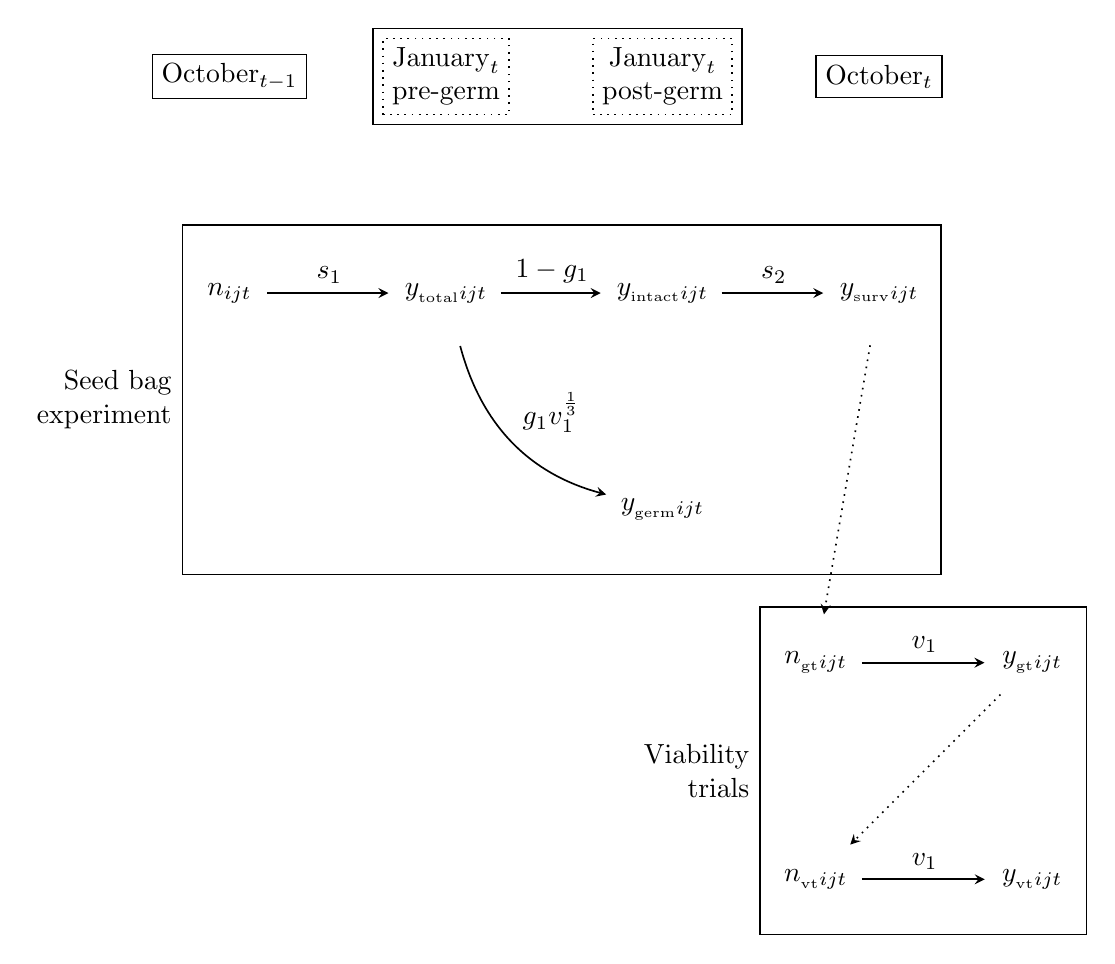
\begin{tikzpicture}[
            > = stealth, % arrow head style
            shorten > = 1pt, % don't touch arrow head to node
            auto,
            node distance = 2.75cm, % distance between nodes
            semithick % line style
        ]

        \tikzstyle{every state}=[
            draw = none,
            thick,
            fill = white,
            minimum size = 4mm
        ]

        \node[state] (Y1a) [] {$y_{_{\mathrm{total}} ijt}$};
        \node[state] (Y1b) [right of=Y1a] {$y_{_{\mathrm{intact}} ijt}$};
        \node[state] (N) [left of=Y1a] {$n_{ijt}$};
        \node[state] (Y2) [right of=Y1b] {$y_{_{\mathrm{surv}} ijt}$};
        \node[state] (G) [below of=Y1b] {$y_{_{\mathrm{germ}} ijt}$};
     
        \node[draw] (O1) [above of=N] {$\mathrm{October}_{t-1}$};
        \node[draw,dotted] (J1) [above of=Y1a, align=center] {$\mathrm{January}_{t}$ \\ pre-germ};
        \node[draw,dotted] (J2) [above of=Y1b, align=center] {$\mathrm{January}_{t}$ \\ post-germ};
        \node[draw,fit=(J1) (J2)] {};
        \node[draw] (O2) [above of=Y2] {$\mathrm{October}_{t}$};

        \path[->] (N) edge node {$s_1$} (Y1a);
        \path[->] (Y1a) edge node {$1-g_1$} (Y1b);
   	\path[->] (Y1b) edge node {$s_2$} (Y2);
       	\path[->] (Y1a) edge[bend right] node {$g_1 v_1^{\frac{1}{3}}$} (G);

        \node[state] (T1) [below right of=G] {$n_{_{\mathrm{gt}} ijt}$};
   	\path[dotted, ->] (Y2) edge node {} (T1);
        \node[state] (TG) [right of=T1] {$y_{_{\mathrm{gt}} ijt}$};
   	\path[->] (T1) edge node {$v_1$} (TG);
        \node[state] (T2) [below of=T1] {$n_{_{\mathrm{vt}} ijt}$};
   	\path[dotted, ->] (TG) edge node {} (T2);
        \node[state] (VG) [right of=T2] {$y_{_{\mathrm{vt}} ijt}$};
   	\path[->] (T2) edge node {$v_1$} (VG);
	
	\node[draw,fit=(N) (Y1a) (Y1b) (Y2) (G) , label={[label distance=0cm, align = right]left:{Seed bag \\ experiment}}] {};
	
	\node[draw,fit=(T1) (T2) (TG) (VG), label={[label distance=0cm, align = right]left:{Viability \\ trials}}] {};

  \end{tikzpicture}
  \caption{Diagram of data from the seed bag experiments and viability trials.}\label{figure1}
 \label{fig:seedBagDiagram}
\end{figure}

\subsection*{Seed survival and germination model}

Overall, the aim of the model is to combine the estimates of seed survival and germination that we obtained from the seed burial experiment in the field with the viability data from the lab trials. 

\subsubsection*{Model for viability trial data}

Each bag $i$ from site $j$ in year $k$ had $h$ trials. The problem is most bags only had 2 trials so it's difficult to estimate a variance. I want to estimate a bag-specific viability because that is what I would use in the seed bag survival and germination model to put a bag-specific viability rather than a site-specific viability. I fit the following model for trial $h$ for bag $i$ at site $j$ in year $k$:
%
\begin{align}
  \begin{split}
 [\bm{\alpha} | & \bm{n}, \bm{n_{\mathrm{gt}}}, \bm{n_{\mathrm{vt}}}, \bm{y_{\mathrm{gt}}},  \bm{y_{\mathrm{vt}}} ] \propto
 \\  & \prod_{j=1}^{J} \prod_{i=1}^{I}  \prod_{h=1}^{H} \prod_{k=1}^{K}  \mathrm{binomial} ( y^{\mathrm{gt}}_{hijk} | n^{\mathrm{gt}}_{hijk}, \mathrm{logit}^{-1}(\alpha_{ijk}) )
 \\ & \times \mathrm{binomial} ( y^{\mathrm{vt}}_{hijk} | n^{\mathrm{vt}}_{hijk}, \mathrm{logit}^{-1}(\alpha_{ijk})  ) 
   \\ & \times \mathrm{normal} ( \alpha_{ijk}  | \mu_{jk}, \sigma_{jk} )
  \\ & \times \mathrm{normal} ( \mu_{jk} | 0 , 100 ) \mathrm{uniform} ( \sigma_{jk} | 0,100)
  \end{split}
\end{align}

I started considering applying the probabilities from the conditional probability tree. This might make sense but then I realize that I've gone down this rabbit hole before. Not all of the seeds that didn't germinate were tested. But I'm not sure how else to control for that besides....

Where P(V) = P(V|Gc)*P(Gc) + P(V|G)*P(G)

\subsubsection*{Model for seed burial experiment data}

To estimate the survival and germination of seeds in each population, I fit the following model for bag $i$ at site $j$ in year $k$. 
%
\begin{align}
  \begin{split}
 [ \bm{\phi}, \bm{\gamma}, \bm{\rho}, \bm{\alpha} | & \bm{n}, \bm{n_{\mathrm{viab}}}, \bm{y_{\mathrm{total}}},  \bm{y_{\mathrm{germ}}},  \bm{y_{\mathrm{surv}}}, \bm{y_{\mathrm{viab}}} ] \propto \\
   & \prod_{j=1}^{J} \prod_{i=1}^{I} % \prod_{k=1}^{K}  
   \mathrm{binomial} ( y^{\mathrm{tot}}_{ij} | n_{ij}, \mathrm{f}_1(\alpha^{s1}_{0,j} , \beta^{s1}_{j} ) ) 
 \\ & \times \mathrm{binomial} ( y^{\mathrm{germ}}_{ij}  | y^{\mathrm{tot}}_{ij}  , \mathrm{f}_2( \gamma_{j} , \alpha_{ijk}) )
 \\ & \times \mathrm{binomial} ( y^{\mathrm{surv}}_{ij} | y^{\mathrm{tot}}_{ij}  -  y^{\mathrm{germ}}_{ij}   , \mathrm{f}_3(\alpha^{s2}_{0,j} , \beta^{s2}_{j} ) ) 
 \\ & \times  \mathrm{binomial} ( y^{\mathrm{viab}}_{ij} | n^{\mathrm{viab}}_{ij}, \mathrm{logit}^{-1}(\alpha_{ijk}) ) 
    \\ & \times \mathrm{normal} ( \alpha^{s1}_{0,j} | 0, 10) \mathrm{normal} ( \alpha^{g1}_{0,j} | 0, 10) \mathrm{normal} ( \alpha^{s2}_{0,j} | 0, 10)  
    \\ & \times \mathrm{normal} ( \beta^{s1}_{j} | 0, \sigma_j^{s1}) \mathrm{normal} ( \beta^{g1}_{j} | 0, \sigma_j^{g1}) \mathrm{normal} ( \beta^{s2}_{j} | 0, \sigma_j^{s2}) 
    \\ & \times \mathrm{uniform} ( \sigma_j^{s1} | 0, 100) \mathrm{uniform} ( \sigma_j^{g1} | 0, 100)  \mathrm{uniform} ( \sigma_j^{s2} | 0, 100)   
  \\ & \times \mathrm{normal} ( \alpha_{ijk}  | \mu_{jk}, \sigma_{jk} )
  \\ & \times \mathrm{normal} ( \mu_{jk} | 0 , 100 ) \mathrm{uniform} ( \sigma_{jk} | 0,100).
  \end{split}
\end{align}
%
where
%
\begin{align}
  \begin{split}
\mathrm{f}_1(\alpha^{s1}_{0,j} , \beta^{s1}_{jk} ) ) & =  \phi_{jk} = \mathrm{logit}^{-1}(\alpha^{s1}_{0,j} + \beta^{s1}_{jk}) \\
\mathrm{f}_2(\alpha^{g1}_{0,j} , \beta^{g1}_{jk},  \alpha_{ijk} ) ) & = \gamma_{jk} \times v_{ijk}^\frac{1}{3} = \mathrm{logit}^{-1}(\alpha^{s1}_{0,j} + \beta^{s1}_{jk}) \times ( \mathrm{logit}^{-1}(\alpha_{ijk}))^\frac{1}{3} \\
\mathrm{f}_3(\alpha^{s2}_{0,j} , \beta^{s2}_{jk} ) ) & =  \rho_{jk} = \mathrm{logit}^{-1}(\alpha^{s1}_{0,j} + \beta^{s1}_{jk})
  \end{split}
\end{align}



I fit this model with JAGS in R. %In order to evaluate the effect of the prior, we obtained estimates for all parameters with a noninformative beta(1,1) prior and the informative prior on the logit transformed $\alpha$ parameter. In the derived quantities block, we calculated the dormancy for each bag $(1-g)*v$. Question is how to get dormancy for the site because viability is bag level. We simulate data from this model and calculate test statistics.

\subsubsection*{Full model}

To estimate the survival and germination of seeds in each population, I fit the following model for bag $i$ at site $j$ in year $k$:
%
\begin{align}
  \begin{split}
 [ \bm{\phi}, \bm{\gamma}, \bm{\rho}, \bm{\alpha} | & \bm{n}, \bm{n_{\mathrm{viab}}}, \bm{y_{\mathrm{total}}},  \bm{y_{\mathrm{germ}}},  \bm{y_{\mathrm{surv}}}, \bm{y_{\mathrm{viab}}} ] \propto \\
   & \prod_{j=1}^{J} \prod_{i=1}^{I} % \prod_{k=1}^{K}  
   \mathrm{binomial} ( y^{\mathrm{tot}}_{ij} | n_{ij}, \mathrm{f}_1(\alpha^{s1}_{0,j} , \beta^{s1}_{j} ) ) 
 \\ & \times \mathrm{binomial} ( y^{\mathrm{germ}}_{ij}  | y^{\mathrm{tot}}_{ij}  , \mathrm{f}_2( \gamma_{j} , \alpha_{ijk}) )
 \\ & \times \mathrm{binomial} ( y^{\mathrm{surv}}_{ij} | y^{\mathrm{tot}}_{ij}  -  y^{\mathrm{germ}}_{ij}   , \mathrm{f}_3(\alpha^{s2}_{0,j} , \beta^{s2}_{j} ) ) 
 \\ & \times  \mathrm{binomial} ( y^{\mathrm{viab}}_{ij} | n^{\mathrm{viab}}_{ij}, \mathrm{logit}^{-1}(\alpha_{ijk}) ) 
    \\ & \times \mathrm{normal} ( \alpha^{s1}_{0,j} | 0, 10) \mathrm{normal} ( \alpha^{g1}_{0,j} | 0, 10) \mathrm{normal} ( \alpha^{s2}_{0,j} | 0, 10)  
    \\ & \times \mathrm{normal} ( \beta^{s1}_{j} | 0, \sigma_j^{s1}) \mathrm{normal} ( \beta^{g1}_{j} | 0, \sigma_j^{g1}) \mathrm{normal} ( \beta^{s2}_{j} | 0, \sigma_j^{s2}) 
    \\ & \times \mathrm{uniform} ( \sigma_j^{s1} | 0, 100) \mathrm{uniform} ( \sigma_j^{g1} | 0, 100)  \mathrm{uniform} ( \sigma_j^{s2} | 0, 100)   
  \\ & \times \mathrm{normal} ( \alpha_{ijk}  | \mu_{jk}, \sigma_{jk} )
  \\ & \times \mathrm{normal} ( \mu_{jk} | 0 , 100 ) \mathrm{uniform} ( \sigma_{jk} | 0,100).
  \end{split}
\end{align}
%
where
%
\begin{align}
  \begin{split}
\mathrm{f}_1(\alpha^{s1}_{0,j} , \beta^{s1}_{jk} ) ) & =  \phi_{jk} = \mathrm{logit}^{-1}(\alpha^{s1}_{0,j} + \beta^{s1}_{jk}) \\
\mathrm{f}_2(\alpha^{g1}_{0,j} , \beta^{g1}_{jk},  \alpha_{ijk} ) ) & = \gamma_{jk} \times v_{ijk}^\frac{1}{3} = \mathrm{logit}^{-1}(\alpha^{s1}_{0,j} + \beta^{s1}_{jk}) \times ( \mathrm{logit}^{-1}(\alpha_{ijk}))^\frac{1}{3} \\
\mathrm{f}_3(\alpha^{s2}_{0,j} , \beta^{s2}_{jk} ) ) & =  \rho_{jk} = \mathrm{logit}^{-1}(\alpha^{s1}_{0,j} + \beta^{s1}_{jk})
  \end{split}
\end{align}

These models relate the average seed survival in each population to the seed survival observed in a given year through a linear model. The function has a parameter for the average seed survival in each population, and a parameter for the seed survival of each population in each year. I treated seed survival as a binomially-distributed random variable because the data come from an experiment in which we buried a known number of seeds and counted seeds. Thus for the $i$th observation, I parameterized a binomial distribution in terms of a probability and a known number of trials. I sampled a 95\% credible interval from the posterior predictive distribution for seed survival for each site and compared it to the seed burial experiments to assess whether the model from the seed burial experiments could predict the seed survival in seed burial experiments. 

I fit this model with JAGS in R. %In order to evaluate the effect of the prior, we obtained estimates for all parameters with a noninformative beta(1,1) prior and the informative prior on the logit transformed $\alpha$ parameter. In the derived quantities block, we calculated the dormancy for each bag $(1-g)*v$. Question is how to get dormancy for the site because viability is bag level. We simulate data from this model and calculate test statistics.

\section*{Seedling survival to fruiting}

The data consist of counts of seedlings and fruiting plants in 0.5 m$^2$ plots at 20 sites from 2006--present. Each site was visited in February and June to count the number of seedlings and fruiting plants, respectively. Seedlings and plants in each plot are counted by a single person at each visit. 

For now, we assume that the data on seedlings is measured perfectly (i.e. no under- or over-counts of seedlings). However, there are at least two possible sources of error: (1) measurement error that arises because we failed to count seedlings that were present and (2) error that arises because seedlings germinated after we visited the site. Germination phenology varies may vary from year to year but also by geography; higher elevation sites may have delayed phenology. We may want to develop a model that relates our estimate of seedlings to the true number of seedlings in a plot because we sometimes observe more fruiting plants than seedlings. For now, I ignored data that involved undercounting by filtering out those rows in the dataset.

We assume that the data on fruiting plants is measured perfectly (i.e. we did not under- or over- count) because plants stand out from the background vegetation in June. Our model estimates the proportion of seedlings that survive to become fruiting plants. Define:

\begin{itemize}
	\item $n_{ijt}$ = observed counts of seedlings in the $i^{th}$ plot, from the $j^{th}$ site, from the $k^{th}$ year
	%\item $z_{ijt}$ = true counts of seedlings in the $i^{th}$ plot, from the $j^{th}$ site, from the $t^{th}$ year
	\item $y_{ijt}$ = observed counts of fruiting plants in the $i^{th}$ plot, from the $j^{th}$ site, from the $k^{th}$ year, assumed to be measured perfectly
\end{itemize}

We estimated survival across all sites taking into account both temporal and between-site variability with the following model. In this model, $\alpha^S_{0,j}$ is the logit mean survival probability at site $j$, $\beta^S_{jk}$ are independent identically distributed random variables drawn from normal distributions with mean 0 and site-specific temporal variance parameters $\sigma_j^S$. Writing the site-specific logit survival as a fixed effect means that each site parameter estimate is estimated separately with no shared variance term. The site-specific temporal variance parameter is written as a random effect, which means that each site has has year components that are drawn from a distribution with a shared variance term. I estimated the probability of surviving to fruiting using data from plots at sites in different years:

\begin{align}
  \begin{split}
 [ \bm{\alpha^S_0}, \bm{\beta^S}, \sigma^S | \bm{n}, \bm{y} ] \propto 
 & \prod_{i=1}^{I} \prod_{j=1}^{J} \prod_{k=1}^{K} \mathrm{binomial} ( y_{ijk} | n_{ijt}, \mathrm{f}(\alpha^S_{0,j} , \beta^S_{jk} ) )
     \\ & \times \mathrm{normal} ( \beta^S_{jk} | 0, \sigma_j^S) 
    \\ & \times \mathrm{normal} ( \alpha^S_{0,j} | 0, 10) \mathrm{uniform} ( \sigma_j^S | 0, 100)  
   \end{split}
\end{align}
%
where

\begin{align}
  \begin{split}
\mathrm{f}(\alpha^S_{0,j} , \beta^S_k ) ) = \mathrm{logit}^{-1}(\alpha^S_{0,j} + \beta^S_{jk})
  \end{split}
\end{align}
%
\subsection*{Fruits per plant}

From 2006--2012, "we recorded...the number of fruits per plant for up to 15-20 plants per 0.5 m$^2$" (\cite{eckhart2011}). For each plant, we counted the number of undamaged fruits. We then took the damaged fruits and visually stacked them end to end to estimate how many additional undamaged fruits that was equivalent to (e.g. two half fruits corresponded to one undamaged fruit). We used these counts to estimate the number fruits produced per plant. 

% From 2013--present, we counted the number of undamaged and damaged fruits per plant for up to ... plants per 0.5 m$^2$. We used these counts to estimate the number of fruits produced per plant, and to estimate the number of those fruits that are damaged by herbivores.

We seek to estimate (1) the number of fruits produced per plant and (2) the proportion of fruits that are damaged per plant. Define: 

\begin{itemize}

	\item $y^{TFE}_{ijk}$ = observed counts of total fruit equivalents per plant on the $i^{th}$ plant, from the $j^{th}$ site, from the $k^{th}$ year, assumed to be measured perfectly
%	\item $\bm{y_{ijk}} = [ y^{und}_{ijt}, y^{dam}_{ijt} ] $ = two item vector of observed counts of undamaged and damaged fruits per plant on the $i^{th}$ plant, from the $j^{th}$ site, from the $k^{th}$ year, assumed to be measured perfectly
	\item $n_{ijk}$ = observed counts of total fruits per plant (sum of $\bm{y_{ijk}}$) on the $i^{th}$ plant, from the $j^{th}$ site, from the $k^{th}$ year, assumed to be measured perfectly
%	\item $\phi_{jt}$ = the true, unobserved proportion of fruits that are damaged per plant at the $j^{th}$ site, in the $k^{th}$ year
\end{itemize}

To assess what probability distribution to use when fitting this model, I fit a power model with an intercept to the mean and variance using the `nls` function in R, which returned an exponent of 1.99. The fit is close to quadratic which means a negative binomial is likely to be an appropriate distribution (\cite{linden2011}). We estimated fruits per plant across all sites taking into account both temporal and between-site variability with the following model. I first worked only with data on total fruit equivalents on a plant (2006-2012). I estimated total fruit equivalents per plant as: 

\begin{align}
  \begin{split}
 [ \bm{\alpha^F_0}, \bm{\beta^F}, \sigma^F | \bm{n}, \bm{y} ] \propto 
 & \prod_{i=1}^{I} \prod_{j=1}^{J} \prod_{k=1}^{K}  \mathrm{negative \ binomial} ( y^{\mathrm{TFE}}_{ijk} | \mathrm{f}_1(\alpha^F_{0,j} , \beta^F_{jk} ),  \kappa^F ) )
     \\ & \times \mathrm{normal} ( \alpha^F_{0,j} | 0, 10) 
     \\ & \times \mathrm{normal} ( \beta^F_{jk} | 0, \sigma^F_j) 
    \\ & \times \mathrm{normal} ( \sigma^F_j | 0, 100)  
   \end{split}
\end{align}
%
where

\begin{align}
  \begin{split}
\mathrm{f}_1(\alpha^F_{0,j} , \beta^F_{jk} ) ) = \lambda^F_{jk} = \mathrm{exp}( \alpha^F_{0,j} + \beta^F_{jk} ) \\
% \mathrm{f}_2(\alpha^F_{0,j} , \beta^F_{jk} ) ) = \kappa^F = \mathrm{exp}( \alpha^F_{0,j} + \beta^F_{jk} )
  \end{split}
\end{align}

\begin{align}
  \begin{split}
  \mathrm{negative \ binomial} ( y^{\mathrm{TFE}}_{ijk} | \frac{\kappa^F}{\kappa^F + \lambda^F_{jk}} ,  \kappa^F )
  \end{split}
\end{align}
%
where the negative binomial is parameterized with probability parameter $p$ and dispersion parameter $r$ [$ \mathrm{negative \ binomial}(p,r)$]. In this case $p=\frac{\kappa}{\kappa+\mu}$.

\subsection*{Seeds per fruit}

From 2006--2012, "we collected one fruit from each of 20-30 haphazardly selected plants distributed across each population (but outside plots, to avoid influencing seed input within them) to estimate the mean number of seeds produced per fruit" (Eckhart et al. 2011). We collected fruits that were undamaged in the field, and fruits were broken open to count seeds. For each population in each year, we attempted to obtain 20-30 counts of seeds produced per undamaged fruit. 

%From 2013--present, we collected one undamaged and one damaged fruit from each of 20-30 haphazardly selected plants distributed across each population. The plants were again outside plots to avoid affecting seed input. We used these fruits to estimate the mean number of seeds produced by undamaged and damaged fruits. Fruits were broken open to count seeds. For each population in each year, we attempted to obtain 20-30 counts of seeds produced per undamaged fruit and  20-30 counts of seeds produced per damaged fruit. 

We seek to estimate (1) the number of seeds per undamaged fruit. Define:

%, (2) the number of seeds per damaged fruit, and (3) the proportion of seeds that are lost to herbivory in damaged fruits relative to undamaged fruits. 

\begin{itemize}
	\item $y^{und}_{ijk}$ = observed counts of seeds per undamaged fruit in the $i^{th}$ fruit, from the $j^{th}$ site, from the $k^{th}$ year, assumed to be measured perfectly
%	\item $y^{dam}_{ijt}$ = observed counts of seeds per damaged fruit in the $i^{th}$ fruit, from the $j^{th}$ site, from the $k^{th}$ year, assumed to be measured perfectly
	\item $\lambda_{jk}$ = true, unobserved mean number of seeds per undamaged fruit from the $j^{th}$ site, from the $k^{th}$ year
\end{itemize}

To assess what probability distribution to use when fitting this model, I fit a power model with an intercept to the mean and variance using the `nls` function in R, which returned an exponent of 1.38. The fit is greater than linear but less than quadratic which means that neither a Poisson nor negative binomial are likely to be entirely appropriate distributions for the data (\cite{linden2011}). I might try the parameterization in that reference but for now I am using the negative binomial because the data are overdispersed. We estimated seeds per fruit across all sites taking into account both temporal and between-site variability with the following model. I first worked only with data from undamaged fruits from the years (2006-2012). I estimated seeds per fruit as: 

\begin{align}
  \begin{split}
 [ \bm{\alpha^P_0}, \bm{\beta^P}, \sigma^P | \bm{n}, \bm{y} ] \propto 
 & \prod_{i=1}^{I} \prod_{j=1}^{J} \prod_{k=1}^{K}  \mathrm{negative \ binomial} ( y^{\mathrm{und}}_{ijk} | \mathrm{f}_1(\alpha^P_{0,j} , \beta^P_{jk} ), \kappa^P ) )
     \\ & \times \mathrm{normal} ( \alpha^P_{0,j} | 0, 10)  \times 
     \\ & \times \mathrm{normal} ( \beta^P_{jk} | 0, \sigma^P_j) 
    \\ & \mathrm{normal} ( \sigma^P_j | 0, 100)  
   \end{split}
\end{align}
%
where

\begin{align}
  \begin{split}
\mathrm{f}_1(\alpha^P_{0,j} , \beta^P_{jk} ) ) = \lambda^P_{jk} = \mathrm{exp}( \alpha^P_{0,j} + \beta^P_{jk} ) \\
% \mathrm{f}_2(\alpha^P_{0,j} , \beta^P_{jk} ) ) = \kappa^P_{jk} = \mathrm{exp}( \alpha^P_{0,j} + \beta^P_{jk} )
  \end{split}
\end{align}

\begin{align}
  \begin{split}
  \mathrm{negative \ binomial} ( y^{\mathrm{und}}_{ijk} | \frac{\kappa^P}{\kappa^P + \lambda^P_{jk}} ,  \kappa^FP)
  \end{split}
\end{align}
%
where the negative binomial is parameterized with probability parameter $p$ and dispersion parameter $r$ [$ \mathrm{negative \ binomial}(p,r)$]. In this case $p=\frac{\kappa}{\kappa+\mu}$.

\subsection*{Correlation between germination probability and variance in per-capita reproductive success}

I assessed whether the observed germination probability was negatively correlated with variance in per-capita reproductive success (\cite{venable2007}). Reproductive success $F_{jk}$ at site $j$ in year $k$ was calculated at the per year and per site level as follows:

\begin{align}
  \begin{split}
F_{jk} = \phi_{jk} \times \lambda^F_{jk} \times \lambda^P_{jk}
  \end{split}
\end{align}
%
where

\begin{align}
  \begin{split}
\phi_{jk} & = \mathrm{logit}^{-1}(\alpha^S_{0,j} + \beta^S_{jk}) \\
\lambda^F_{jk} & = \mathrm{exp}(\alpha^F_{0,j} + \beta^F_{jk}) \\
\lambda^P_{jk} & = \mathrm{exp}(\alpha^P_{0,j} + \beta^P_{jk}) \\
  \end{split}
\end{align}
%
To calculate the temporal variation in fitness for each population, I sampled the posterior distribution of reproductive success for each year and calculated the geometric SD of per capita reproductive success. For each population, I obtained a posterior distribution for the geometric SD of per capita reproductive success; I used this and the posterior distribution of germination probability from model XX to calculate the correlation between germination and fitness variance. Using this approach, I obtained a distribution of correlation estimates. Results of this analysis are shown in Figure~\ref{fig:germ_rs_correlation}. Bet hedging models predict that germination probability should be negatively correlated with temporal variance in fitness; 95\% credible intervals that do not overlap zero provide support for this prediction.

\subsection*{Correlation between germination probability and seed survival}

I assessed whether the observed germination probability was negatively correlated with seed survival (\cite{gremer2014}). I calculated seed survival as $s_2 s_3$ as the product of these vital rates is the probability that seeds which do not germinate in January remain in the seed bank until the following January. I used the posteriors of $g_1$ and $s_2 s_3$ to calculate the correlation between germination and seed survival. Using this approach, I obtained a distribution of correlation estimates. Results of this analysis are shown in Figure~\ref{fig:germ_surv_correlation}. Bet hedging models predict that germination probability should be negatively correlated with seed survival; 95\% credible intervals that do not overlap zero provide support for this prediction.

\subsection*{Density-independent model for germination probability}

We used estimates of seed survival and reproductive success to investigate the adaptive value of delayed germination (\cite{gremer2014}). Briefly, we parameterize a model of population growth rate and calculate the optimal germination strategy for different combinations of seed survival and reproductive success. We use the following equation to summarize \textit{Clarkia xantiana}'s life cycle and calculate population growth rate:

\begin{align}
  \begin{split}
\lambda_{j} = g_1 Y(t) s_0 s_1 + (1-g_1) s_2 s_3 
  \end{split}
\end{align}
%
The parameters in this equation were fit in models corresponding to equations (1, 3, 5, 8). Seed survival rates ($s_0, s_1, s_2, s_3$) are population-level estimates. Per capita reproductive success ($Y(t)$) is calculated as the product of seedling survival to fruiting, fruits per plant, and seeds per fruit. Variation is incorporated into the model by having $Y(t)$ vary between years.

I numerically calculated the optimal germination probability for the observed level of variation in reproductive success and seed survival in each population. For each population, I randomly selected values 1000 from the posterior distribution for reproductive success. I used this same sequence of $Y(t)$ and the observed seed survival probabilities to calculate long-term stochastic population growth rates ($\lambda_s$) at each germination probability along an evenly spaced grid of possible germination probabilities (G) between 0 and 1. The optimal germination probability is estimated as the value of G that maximized geometric mean of the population growth rate. I repeated the simulations 50 times for each population, resampling from the posterior distribution for reproductive success each time. I calculated the mean of the optimal germination fractions. 

A model in which per-capita reproductive success is density-independent predicts that germination probability should respond to variance in fitness (\cite{cohen1966}). To evaluate a density-independent model for germination probability, I compared observed germination probability to predicted germination optima. I plot this comparison in Figure~\ref{fig:obs_pred}. The dotted line indicates a 1:1 relationship between observations and predictions. Values below the line indicate that the model predicts higher germination probabilities than observed; values above the line would indicate that the model predicts lower germination probabilities than observed.

\section*{Results}

\begin{figure}
\centering
\begin{subfigure}[h]{.65\textwidth}
\centering
       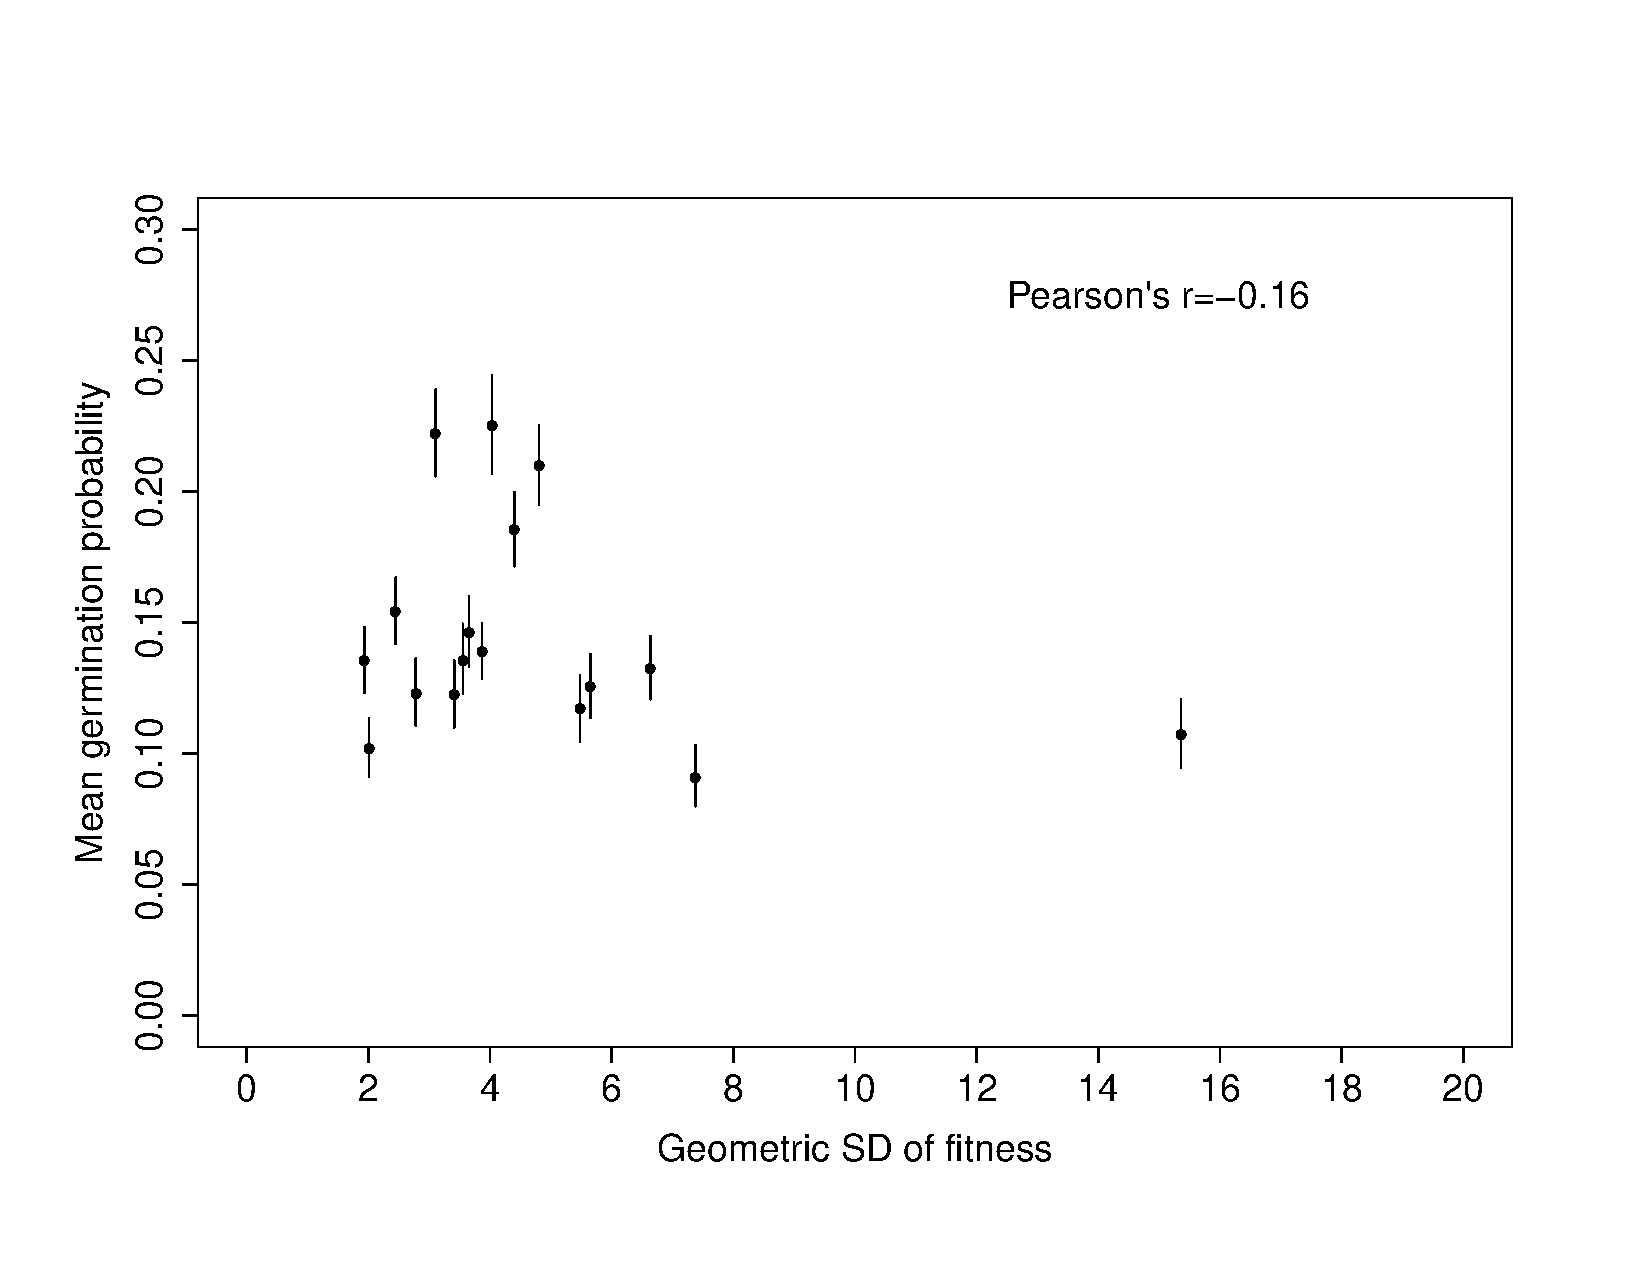
\includegraphics[page=1,width=1\textwidth]{../figures/germ_rs_correlation.pdf}  
\end{subfigure}
\begin{subfigure}[h]{.9\textwidth}
\centering
       \includegraphics[page=2,width=1\textwidth]{../figures/germ_rs_correlation.pdf}  
\end{subfigure}
 \caption{ The top panel shows the observed germination probability plotted against the temporal variation in per capita reproductive success. The bottom panel shows the posterior distribution of correlation between observed germination probability and geometric SD of per capita reproductive success; the median correlation is negative (-0.16) but the 95\% credible interval overlaps 0. }
   \label{fig:germ_rs_correlation}
 \end{figure}

 
 \begin{figure}
\centering
\begin{subfigure}[h]{.65\textwidth}
\centering
       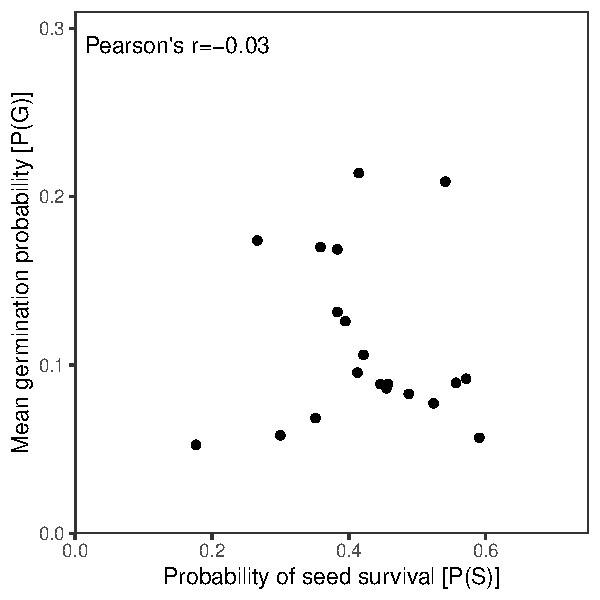
\includegraphics[page=1,width=1\textwidth]{../figures/germ_surv_correlation.pdf}  
\end{subfigure}
\begin{subfigure}[h]{.9\textwidth}
\centering
       \includegraphics[page=2,width=1\textwidth]{../figures/germ_surv_correlation.pdf}  
\end{subfigure}
 \caption{ The top panel shows the observed germination probability plotted against probability of seed survival. The bottom panel shows the posterior distribution of correlation between observed germination probability and the probability of seed survival; the median correlation is negative (-0.16) and the 95\% credible interval does not overlap 0. }
  \label{fig:germ_surv_correlation}
 \end{figure}
 
 \begin{figure}[h]
   \centering
  %#\begin{tabular}{@{}c@{\hspace{.5cm}}c@{}}
       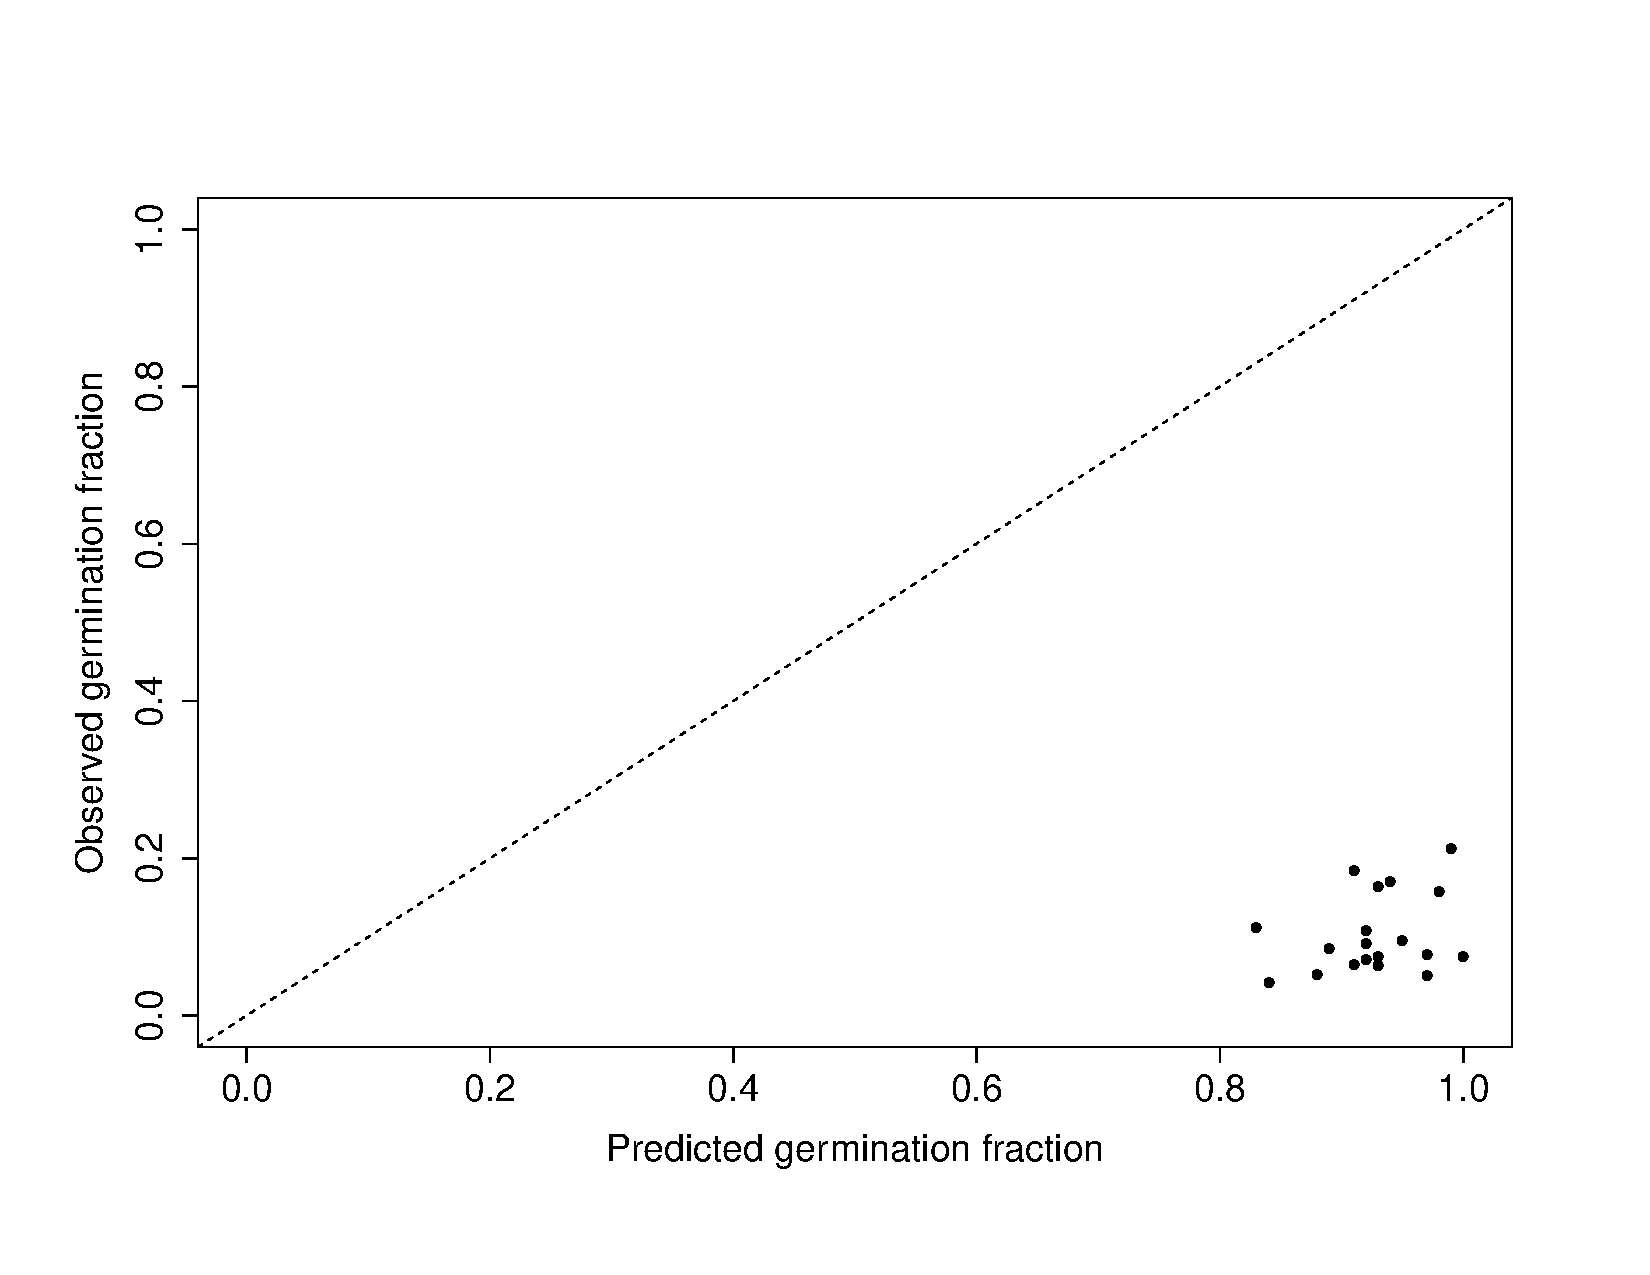
\includegraphics[page=1,width=.9\textwidth]{../figures/obs_pred_germ.pdf}  
    \caption{ Observed germination probability plotted against the optimal germination probability predicted by a density-independent model. For each population, the observed germination probability is the obtained from the model for seed bank vital rates. Each point is the population-specific median of the posterior of $g_1$ for a model fit to data from seed bag experiments from 2006--2009. Data was pooled across years. The dotted line indicates a 1:1 relationship between observations and predictions. Values below the line indicate that the model predicts higher germination probabilities than observed; values above the line would indicate that the model predicts lower germination probabilities than observed. }
 \label{fig:obs_pred}
\end{figure}

\clearpage
\bibliography{/Users/gregor/Dropbox/bibliography/seeds}

\end{document}